\chapter{Objetivos del proyecto}
Este capítulo se ha dividido en tres partes, en la primera se hablará del punto de partida donde comenzó el proyecto. En la segunda parte, se detallarán el alcance y las tecnologías usadas. Y para finalizar, se hará un repaso de las exclusiones que se han identificado dentro del proyecto.
\section{Antecedentes del proyecto}
\label{secc:Antecedentes}
Es común que durante la etapa de la universidad la organización sea un factor muy importante. El tema de la organización para muchos estudiantes suele ser molesta, ya que no les gusta estar apuntando cada tarea que tienen que realizar, ya sean exámenes, notas, horarios, etc, prefieren hacer uso de su memoria y apuntar todo lo que tienen que hacer al cabo del día. Por este motivo, se planteó hacer una aplicación de móvil para evitar tener que estar llevando la agenda siempre encima y poder usar la memoria para las asignaturas de la carrera.
El motivo por el que se fue a desarrollar una aplicación para Android, era aprender más sobre las tecnologías móviles y el desarrollo de un proyecto con usuarios. En la carrera ya se comenzó a impartir algunos trabajos para fomentar el desarrollo con Android, por esto se decidió seguir formándose en ese sistema.

El área de los Smartphones cada vez tiene más fuerza en la sociedad, y es raro no ver a gente por la calle escuchando música con su móvil o chateando. Se quiso juntar la idea presentada antes de la organización junto con los dispositivos móviles. En ese momento surgió la idea de crear una agenda universitaria dentro del móvil. Los usuarios podrían llevar siempre los exámenes al día y tenerlos accesibles sin tener que estar cargando con apuntes y cuadernos.

Un punto a tener en cuenta era, el carácter social que se quería conseguir  mediante la aplicación. Por muchas aplicaciones que hubiera en Internet para el móvil ninguna tenía el nivel social de compartir que se buscaba. Por ese motivo se decidió crear Baldugenda, una aplicación para móviles Android que sirviera como agenda para universitarios, y que se pudiera relacionar la aplicación con otras personas. Android es uno de los sistemas operativos para móviles con mayor tasa de usuarios en el mercado, ésta fue una de las causas por las que se decidió usar Android junto con su  IDE Android Studio. Google ha conseguido que gran parte de los desarrolladores dejen de usar Eclipse, y se pasen a esta nueva IDE tanto por su manejo sencillo, como por las facilidades que ofrece a la hora de crear nuevos proyectos. Android Studio fue la opción escogida para desarrollar Baldugenda.  

Ya se ha hablado en anteriores puntos de esta sección sobre Google, esta empresa tiene mucha importancia dentro de Baldugenda, se ha querido que la aplicación se relacione bien en el ecosistema de Google, por ello los servicios usados fueron la mayoría de esta empresa.
Google es una multinacional que ofrece servicios relacionados con Internet,software y otras tecnologías. Google es dueño de Android, por dicho motivo los servicios de Google se relacionan muy bien con las aplicaciones que se quieran crear en Android. Ésta tiene distintos servicios, por una parte los servicios de organización como Gmail, Keep, Calendar y Drive, y por otra parte los de entretenimiento, Youtube, Chrome, etc.
El aspecto social que propone Baldugenda es poder compartir calendarios con los compañeros de clase mediante Google Calendar. Mediante esta aplicación el usuario puede llevar las notas de los exámenes al día, no tener que realizar suma de notas en cada asignatura y también crear una agenda compartida de los exámenes que hay en común.
Después de los motivos que llevaron a realizar Baldugenda, el objetivo marcado que se tenía que cumplir la aplicación era que lograra ser una agenda para universitarios en formato móvil donde los usuarios podrían apuntar los exámenes y las asignaturas, y al crear los exámenes poder compartirlos por medio de Google Calendar y llevar el al día las notas que se van sacando en una asignatura. 
\newpage
\section{Alcance del proyecto}
\label{secc:Alcance}

Ya se han comentado los motivos por los que se decidió crear Baldugenda, en este apartado se describen las características del problema resuelto, y por otro lado los detalles acerca de las aplicaciones desarrolladas.
Asimismo, se desarrollarán más en profundidad aspectos como la creación de exámenes y asignaturas, la visualización de éstas y otras funcionalidades que se pueden realizar con Baldugenda.
A continuación se detallan los problemas a los que Baldugenda ha dado solución:

\begin{itemize}
	\item El usuario podrá crear asignaturas indicando un nombre, el tipo de evaluación que seguirá en la asignatura, la puntuación máxima  y si desea podrá añadir enlaces.
	\item Estas asignaturas tendrán asociado una serie de exámenes que el usuario podrá crear. Para crear un examen el usuario tendrá que indicar el nombre de dicho examen, a qué asignatura pertenece. En el caso de que se haya dado permiso a Google Calendar se tendrá que seleccionar en qué calendario se guardará el examen, también tendrá que indicar la fecha y la hora que será el examen y la nota sobre la que se evaluará.
	\item El usuario podrá visualizar tanto los exámenes como las asignaturas de manera individual o en forma de lista.
	\item También podrá realizar modificaciones y borrados de las asignaturas o exámenes que quiera.
	\item En el caso de haber creado el examen asociado a un calendario de Google, el usuario podrá acceder al evento creado mediante Baldugenda a través de la aplicación de Google Calendar.
	\item Entrando a la actividad de Backup, el usuario podrá realizar una exportación de la base de datos de Baldugenda a la carpeta que se quiera de Google Drive. También tendrá la opción de importar una base de datos existente ubicada en Google Drive
	\item Mediante la actividad de Calendarios podrá realizar modificaciones sencillas sobre sus propios calendarios de Google Calendar.
	\item El usuario tendrá una opción de ayuda donde se podrá poner en contacto con el desarrollador de Baldugenda mediante e-mail o número de teléfono. También tendrá acceso a la carpeta de Google Drive donde habrá un resumen de las funcionalidades.
	\item Dentro de Baldugenda se podrá seleccionar qué cuenta se quiere usar de Google Calendar y en qué cuenta de Google Drive se quiere realizar la exportación.
\end{itemize}

El desarrollo de las aplicaciones creadas se ha realizado de la siguiente manera:

\begin{enumerate}
	\item Existirá un cliente nativo para dispositivos Android, dicho cliente estará accesible mediante el Play Store de Google con el nombre \href{https://play.google.com/store/apps/details?id=com.mikel.agenda&hl=es}{Baldugenda}.
	\item La aplicación Android podrá ejecutarse a partir de la versión 2.3.3 de este sistema operativo, que a fecha de finalización de esta memoria los dispositivos con esta versión suponen el 99\% del total. Si se quiere usar todo las funcionalidades de la aplicación se necesitará disponer de conexión a Internet.
	\item Las implementaciones se realizarán dando prioridad a tecnologías ya conocidas y con las que se ha trabajado anteriormente.
	\item Se usarán las cuentas de Google vinculadas a los servicios de Google Calendar y Google Drive para acceder a la información que precise la aplicación. Si fuera necesario realizar funcionalidades nuevas se usarían servicios de Google para compatibilizar los ya implementados.
\end{enumerate}
\newpage
\section{Exclusiones del proyecto}
\label{secc:Exclusiones}

Se han excluido del alcance del proyecto los siguientes puntos:

\begin{enumerate}
	\item La justificación de alternativas de las tecnologías elegida para la realización de este proyecto. 
	\item El análisis de carácter legal que resultaría necesario en una aplicación final. La aplicación realiza una importante recogida de datos personales (Asignaturas y Exámenes de un usuario) que se almacenan en el dispositivo y que posteriormente se envían a Google.También se ha recogido información referente a los usuarios que han realizado las pruebas. Esta recogida requiere de una consideración en las distintas consecuencias legales, sobre todo los relativos a la \acrfull{lopd} y la \acrfull{lssi}, lo cual sería materia suficiente para un Proyecto Fin de Carrera separado.
	\item No se implementará un módulo ni un análisis de la seguridad dentro de la aplicación. Los aspectos de la seguridad cuando la aplicación envíe datos a servicios de Google, estos recaerán en su seguridad ya implementada.
	\item La implementación de funcionalidades nuevas que facilitarán el uso de la aplicación a personas con alguna discapacidad, como podría ser la creación de exámenes mediante la voz. 
	\item El desarrollo de cliente distinto a Android.
	\item La implementación de un módulo propio para la autenticación de los usuarios, que se ha delegado en un servicio externo.
\end{enumerate}
\newpage
\section{Objetivo en imágenes}
\label{secc:Objetivo en imágenes}

En las imágenes de la izquierda vemos como el Balduser intenta llevar al día los exámenes sin utilizar ningún tipo de tecnología especial exceptuando el papel y el bolígrafo, por ello se ve afectado al tener que realizar modificaciones que eran imprevistas.

En las imágenes de la derecha vemos al Balduser usando la aplicación en su dispositivo móvil, lo cual le permite organizar su agenda universitaria mas fácilmente.

\begin{figure} [H]
\captionsetup[subfigure]{labelformat=empty}
 \centering
\begin{tabular}{c|c}
  \subfloat[]{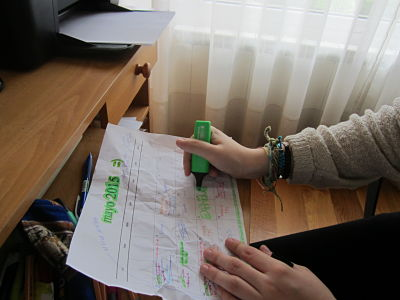
\includegraphics[width=0.5\textwidth]{figs/sin1_opt.png}} & 
  \subfloat[]{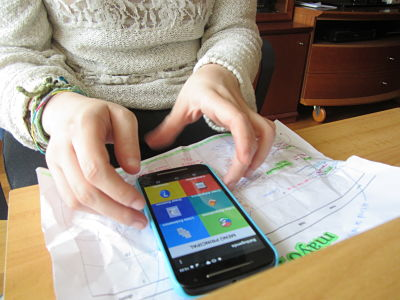
\includegraphics[width=0.5\textwidth]{figs/con1_opt.png}}\\
  \subfloat[]{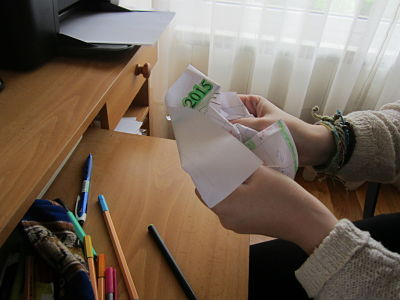
\includegraphics[width=0.5\textwidth]{figs/sin2_opt.png}} & 
  \subfloat[]{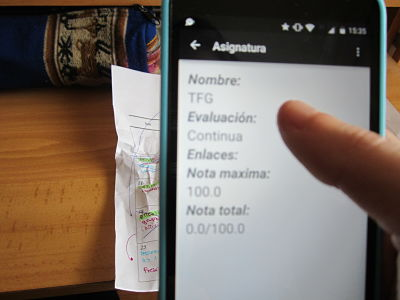
\includegraphics[width=0.5\textwidth]{figs/con2_opt.png}}
  \end{tabular}
 \caption{Objetivo en imágenes}
 \label{f:Objetivo en imágenes}
\end{figure}

